\documentclass[a4paper,10pt]{article}
\usepackage[margin=1in]{geometry}
\usepackage{polski}
\usepackage[utf8x]{inputenc}
\usepackage[unicode]{hyperref}
\usepackage{amssymb}
\usepackage{xifthen}
\usepackage[fleqn]{amsmath}
\usepackage{todonotes}
\usepackage{graphicx}
\usepackage{float}
\usepackage{fullpage}
\usepackage{epstopdf}
\usepackage{multirow}
\usepackage{subfig}
\usepackage[europeanresistors,americaninductors]{circuitikz}
\usetikzlibrary{patterns}
\newcommand{\withtodo}{0}

\def\arraystretch{1.2}

\begin{document}

\begin{table}
  \centering
  \def\arraystretch{1.5}
    \begin{tabular}{|l|l|l|l|} \hline
    Wydział:           & \multicolumn{2}{l|}{Dzień:Poniedziałek 14-17}    &Zespół:  \\
    Fizyki             &    \multicolumn{2}{l|}{Data: 20.03.2017}         &8             \\\hline
    Imiona i nazwiska: &Ocena z przygotowania:  &Ocena ze sprawozdania:   &Ocena końcowa: \\
    Marta Pogorzelska  &                        &                         &                \\
    Paulina Marikin    &                        &                         &\\\hline
    \multicolumn{2}{|l|}{Prowadzący:                 } &\multicolumn{2}{l|}{Podpis:             }  \\\hline
  \end{tabular}
\end{table}

\title{Ćwiczenie 3:\\Wahadło matematyczne}
\date{}
\maketitle{}

\section{Cel badań}
Zbadanie aharmoniczności drgań wahadła matematycznego oraz wyznaczenie wartości przyspieszenia ziemskiego przy użyciu wahadła różnicowego.

\section{Wstęp teoretyczny}
Wahadłem matematycznym jest ciało o masie punktowej m zawieszone na cienkiej, nieważkiej lince o dłuości l poruszającym się po okręgu w jednorodnym polu grawitacyjnym.
\\
\\
\begin{figure}[H]
\centering
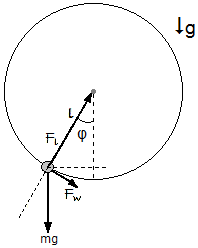
\includegraphics[width=0.3\textwidth]{wahadlo.png}
\end{figure}


\section{Opis układu i metody pomiarowej}

\section{Wyniki pomiarów}

\section{Analiza niepewności}

\section{Wnioski}


\end{document}